\glsresetall

\section{Dog and human inflammatory bowel disease rely on overlapping yet distinct dysbiosis networks}

\subsection{Abstract}

\Gls{ibd} is an autoimmune condition that is difficult to diagnose, and where animal models of this disease have questionable human relevance \cite{RN17324}. Here we show that the dysbiosis network underlying \gls{ibd} in dogs differs from that in humans, with some bacteria such as \textit{Fusobacterium} switching roles between the two species (as \textit{Bacteroides fragilis} switches roles between humans and mice) \cite{RN154}. For example a dysbiosis index trained on humans fails when applied to dogs, but a dog-specific dysbiosis index achieves high correlations with the overall dog microbial community diversity patterns. In addition, a random forests classifier trained on dog-specific samples achieves high discriminatory power, even when using stool samples rather than the mucosal biopsies required for high discriminatory power in humans \cite{RN154}. These relationships were not detected in previously published dog \gls{ibd} datasets due to their limited sample size and statistical power \cite{RN147}. Taken together, these results reveal the need to train host-specific dysbiosis networks and point the way towards a generalized understanding of \gls{ibd} across different mammalian models.

\subsection{Introduction}

Dogs are commonly used as large animal models for drug discovery and safety assessment. The usefulness dogs as a model for \gls{ibd} is yet unexplored, though not unreasonable, as dogs have been useful for studying spontaneously occurring disorders similar to those affecting people \cite{RN144}. For example, dogs live in a close relationship with and share an environment with their owners, and are, therefore, frequently exposed to similar environmental factors, including enteropathogens and toxins. It is well recognized that dogs and humans suffer from similar spontaneous and lifestyle associated diseases such as obesity, allergies, diabetes mellitus, and cancer, and are often treated with similar antibiotics and drugs. \gls{ibd} in humans is a chronic autoimmune disease of multifactorial aetiology and has limited treatment options. Similarly, canine idiopathic \gls{ibd} is a commonly observed chronic inflammatory enteropathy that occurs spontaneously due to similar multifactorial aetiology, namely due to an interplay between an aberrant host immune system, genetics, environmental factors and gut microbiota \cite{RN17324}. Common clinical signs are vomiting, diarrhea, and weight loss. Histological evaluation of intestinal biopsies reveal diffuse or multi-focal inflammatory cell infiltration (most commonly lymphoplasmacytic, followed by eosinophilic and neutrophilic infiltration), with concurrent changes in mucosal architecture (e.g., villus atrophy and fusion) \cite{RN174}. Enteric protein loss may be observed in severe cases. Also, in a subset of dogs, invasive and adherent\textit{ E. coli} have been described, and these share common features with strains isolated from humans with Crohn's disease \cite{RN146}.  Clinical signs may be controlled by single or combination therapy including dietary modifications, antibiotics, and immunosuppressants. However, clinical relapse occurs frequently, and life-long therapy may be needed. Previous small-scale studies have revealed dysbiosis in the small and large intestine of dogs with \gls{ibd}, with some changes in bacterial taxa similar to those observed in humans with \gls{ibd} \cite{RN147}. For example, in both humans and dogs with \gls{ibd}, increases in Proteobacteria, specifically Enterobacteriaceae \cite{RN17268}, and decreases in Firmicutes, including \textit{Faecalibacterium} and \textit{Blautia} \cite{RN17138} have been reported. However, no detailed studies comparing the changes in gut microbiota between humans and canines with \gls{ibd} have been reported to date. The aim of this study was to describe in detail the microbiome changes in a large group of dogs with \gls{ibd}, compare these to the microbiome of humans with \gls{ibd}, assess host similarities and differences, and to train a dysbiosis index composed of non-\gls{ibd} and \gls{ibd} associated bacteria.  

\subsection{Results and Discussion}

As expected based on results from human studies \cite{RN3999, RN154}, but not previously clearly established in canine studies \cite{RN153, RN17138}, dog \gls{ibd} cases and controls differ substantially in both microbial community diversity and structure (Figure~\ref{dogs_fig1}). \gls{ibd} dogs had a significantly lower alpha diversity (Mann-Whitney test, p=0.003) compared to non-\gls{ibd} affected dogs (Figure~\ref{dogs_fig1}A), however alpha diversity in this population did not correlate with age, fat intake, weight, or protein intake (Supplementary Figure~1\footnote{\url{https://images.nature.com/original/nature-assets/nmicrobiol/2016/nmicrobiol2016177/extref/nmicrobiol2016177-s1.pdf}}), nor with body condition scores (p $>$ 0.05, see supplemental methods). Clear separation (using \gls{permanova} grouping samples by disease status, p=0.001 see supplemental methods) between \gls{ibd} dogs and controls was observed using unweighted UniFrac (Figure~\ref{dogs_fig1}B), and the biplot shows the most abundant taxa driving these overall patterns. Consistent with \cite{RN153}; antibiotic history did not reveal differences within \gls{ibd} affected dogs (\gls{permanova} p=0.501, abx=35, no abx=12), on the contrary a significant effect was observed in non-\gls{ibd} dogs (\gls{permanova} p=0.01; abx=8, no abx=77). Finally when combined, the disease effect was significantly stronger (\gls{permanova} p=0.001) than the history of antibiotic usage (pseudo-F on \gls{ibd} groups 1.99 and pseudo-F based on antibiotics groups 9.46; 1.99 $<$ 9.46).

\begin{figure}[htbp]
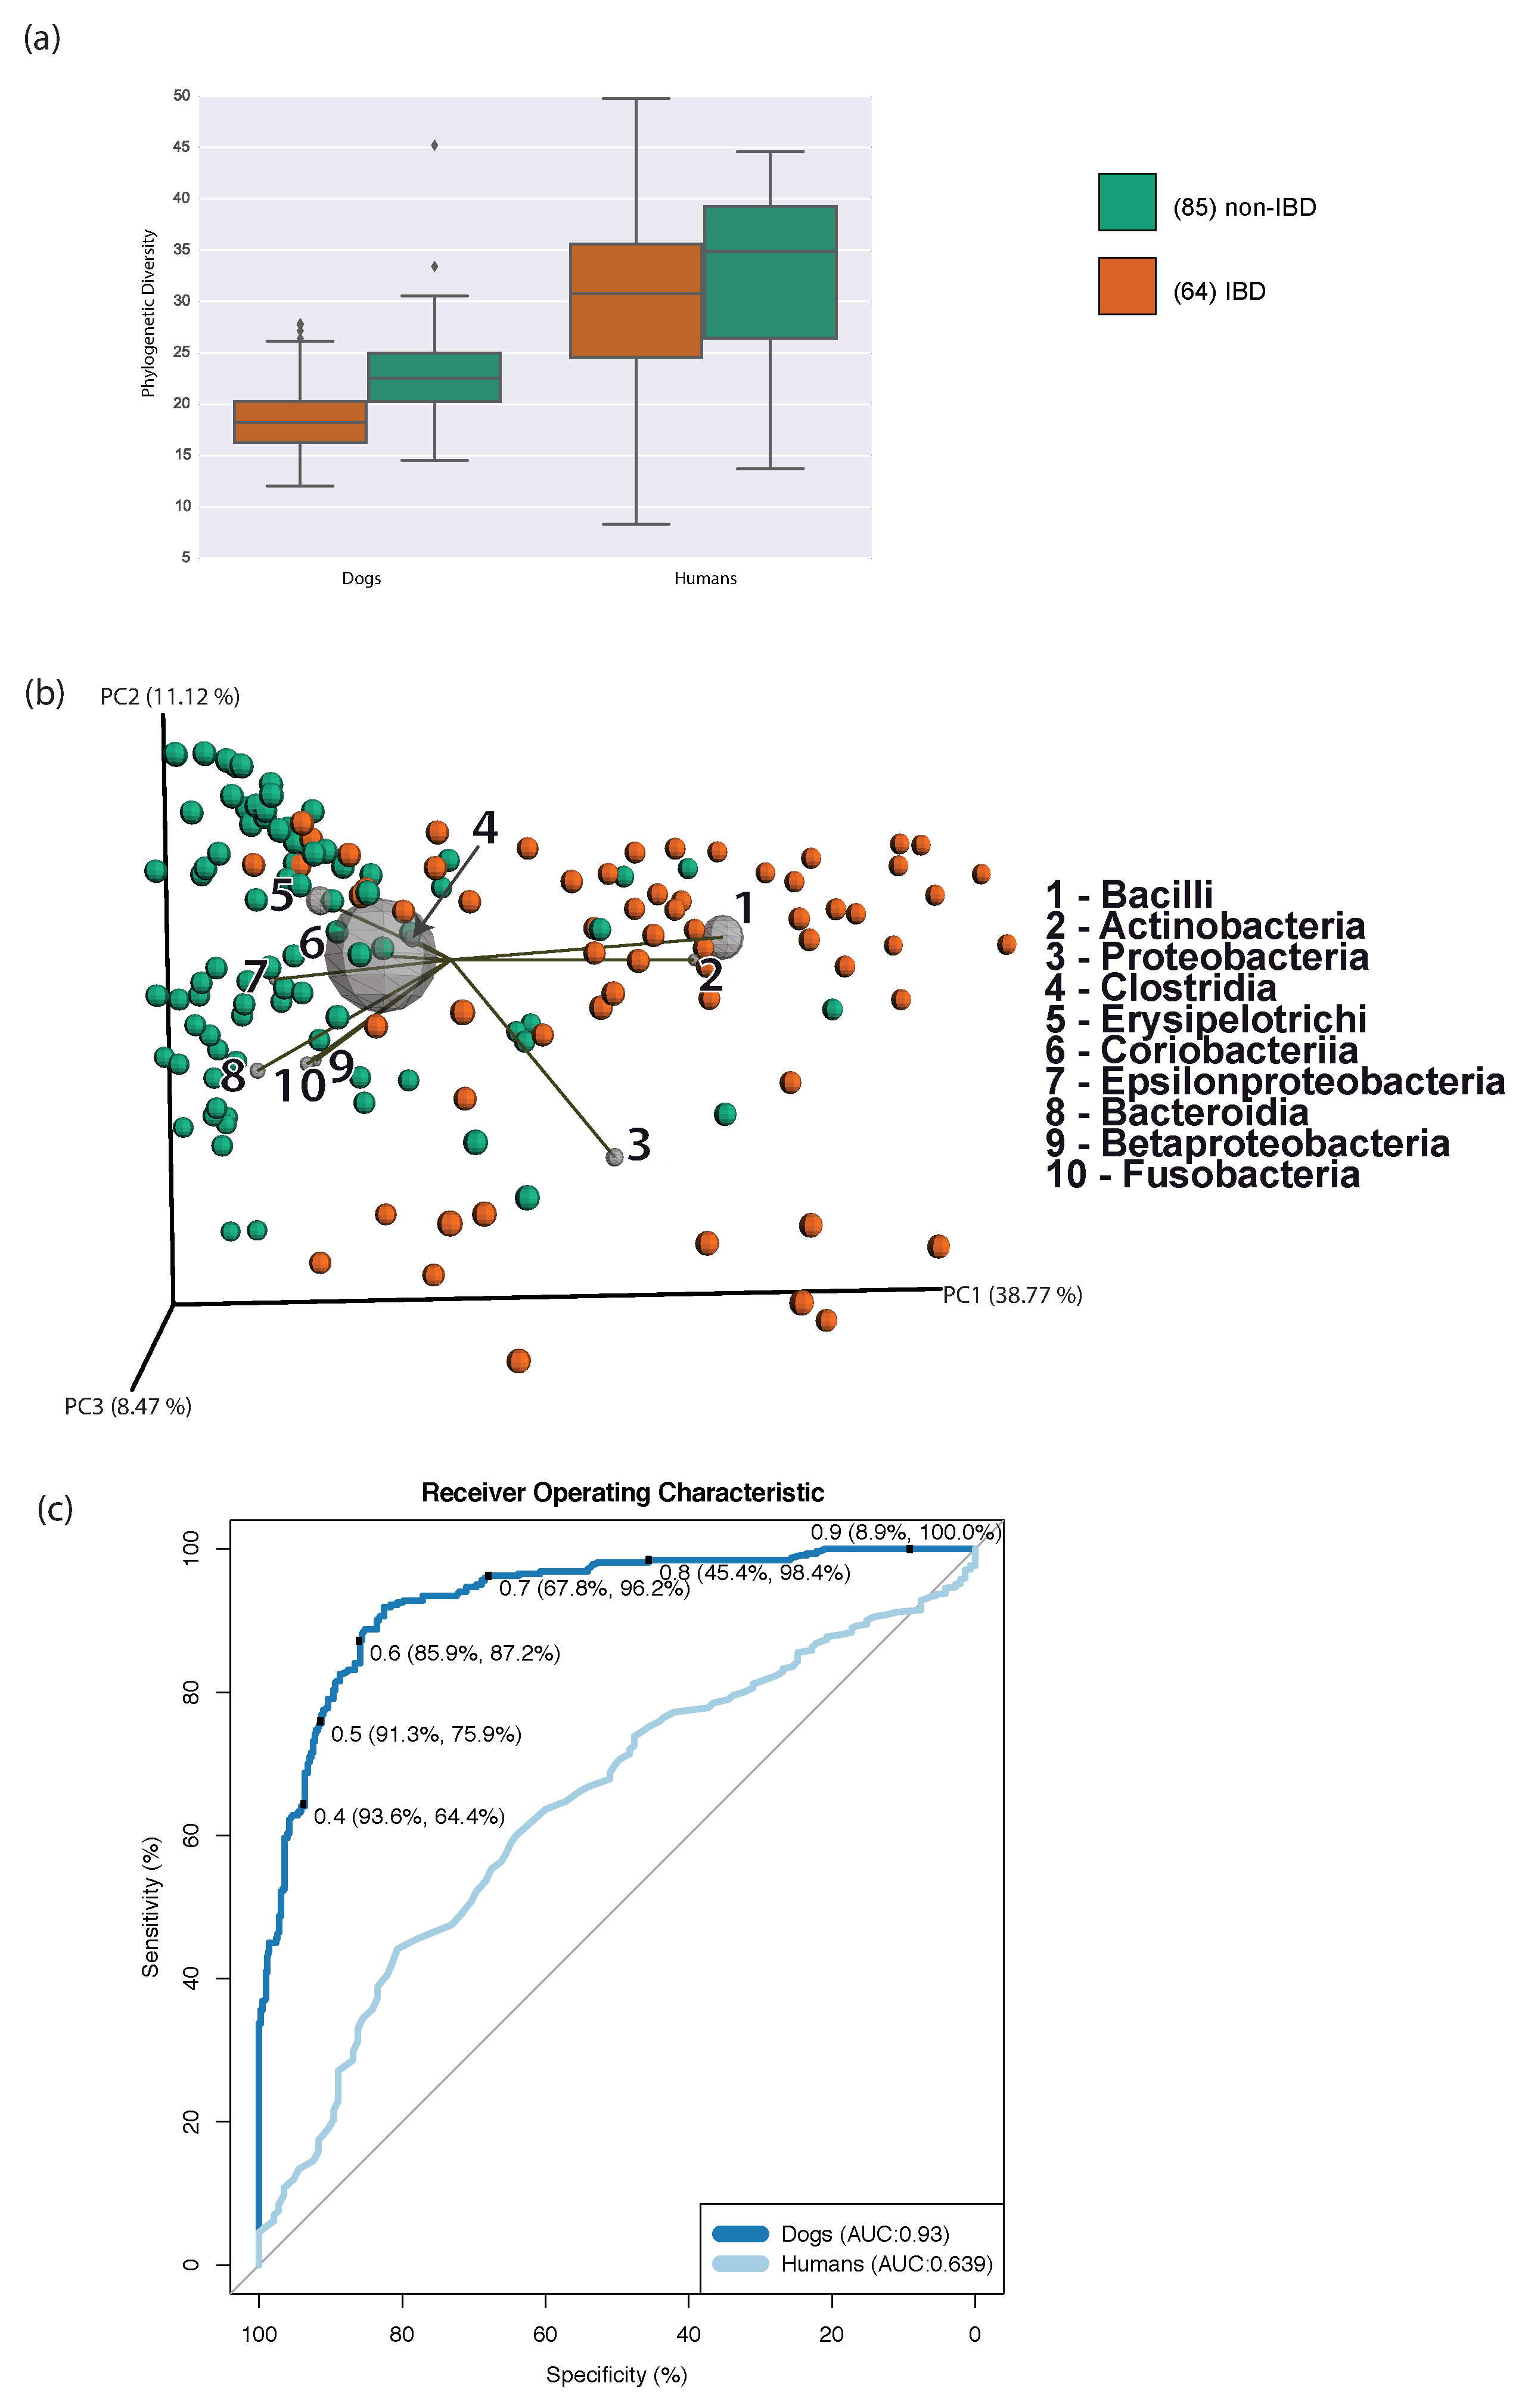
\includegraphics[height=0.85\textheight]{dogs-figures/figure-1}
\label{dogs_fig1}
\caption[Diversity overview and a comparison against humans.]{\textbf{Diversity overview and a comparison against humans.} (a) Comparison between disease states and species of Faith's phylogenetic diversity (whiskers extend for 1.5 times the \gls{iqr} past the low and high quartiles). (b) Weighted UniFrac beta diversity biplot, for the dog samples colored by disease status. (c) Performance comparison of a random forest classifier trained to separate the healthy from the diseased samples in both humans and dogs.}
\end{figure}

A random forests classifier \cite{RN4205} trained on the dog data achieved an \gls{auc} of 0.93 (Figure~\ref{dogs_fig1}C, see discriminant \glspl{otu} in Supplementary Table~1\footnote{\url{https://images.nature.com/original/nature-assets/nmicrobiol/2016/nmicrobiol2016177/extref/nmicrobiol2016177-s1.pdf}}), demonstrating excellent classification accuracy compared to human stool samples where the \gls{auc} was only 0.63 using a much larger training set \cite{RN154}, and achieved only \gls{auc} = 0.86 even using mucosal biopsies. Consequently, in dogs, but not in humans, high classifier accuracy is achievable for \gls{ibd} using only stool samples.

Encouraged by these results, we tested whether a dysbiosis (see supplemental methods) network trained on stool samples alone could be used to interpret the pattern of \gls{ibd} in dogs, and whether this pattern overlapped the human network. We previously found that in humans, substantially better correlation networks could be achieved from the mucosal biopsies, because many taxa contributing to these networks were not seen in stool. Accordingly, we used the techniques described \cite{RN154} to generate correlation networks and a dysbiosis index for dog samples (see supplemental methods for more information). Using the network together with the biplots (Figure~\ref{dogs_fig1}B) we see that Gammaproteobacteria (specifically \textit{Enterobacteriaceae}) were significantly associated with \gls{ibd}, whereas various Firmicutes such as Clostridium and \textit{Ruminococcus} were associated with non-\gls{ibd} samples. When these features are compared with the discriminant \glspl{otu}, obtained from the random forests classifier, we observe a general overlap of the lineages (see Supplementary Table 1 and Supplementary Table 2\footnote{\label{sup}\url{https://images.nature.com/original/nature-assets/nmicrobiol/2016/nmicrobiol2016177/extref/nmicrobiol2016177-s1.pdf}}). However we also see \glspl{otu} that are not highlighted by the correlation network. Specifically Erysipelotrichaceae \textit{Allobaculum} and Lachnospiraceae \textit{Blautia producta}, this is likely because these do not consistently co-occur with or co-exclude other taxa.

The human dysbiosis index failed to negatively correlate with alpha diversity in dog samples (Figure~\ref{dogs_fig2}A.1 and A.2 correlation, A.3 \gls{pcoa} plot), while a dog-specific dysbiosis index showed a statistically significant negative correlation in the same samples (Figure~\ref{dogs_fig2}B.1 and 2 B.2 correlation, C.3 \gls{pcoa} plot, see for a reference the two groups in Figure~\ref{dogs_fig2}D). Additionally we tested the index with previous data \cite{RN153}, and although the sample size is limited, we observed similar patterns (see Supplementary Figure 2\textsuperscript{\ref{sup}}). Similarly to humans, the dysbiosis index in dogs is negatively correlated with phylogenetic diversity (r = -0.45, p $<$ 0.001). However, the list of `non-\gls{ibd}' (co-occurring in non-\gls{ibd} samples) and `\gls{ibd}' (co-occurring in \gls{ibd} samples) bacteria only partially overlaps between host species (see Supplementary Table~2\textsuperscript{\ref{sup}}). Comparing the correlation networks of the taxa for humans (as described in \cite{RN154}) and the network generated for the dog data (Figure~\ref{dogs_fig2}C) revealed overlapping, and discordant taxa. In particular, \textit{Fusobacterium} appears to be associated with \gls{ibd} \cite{RN154} and colorectal cancer \cite{RN3983} in humans but with non-\gls{ibd} dog samples. Of note, we previously observed high levels of \textit{Fusobacterium} sp. in dogs \cite{RN150} but also carnivores of multiple species \cite{RN8250, RN172}, and noted higher levels of \textit{Fusobacterium} in dogs with more access to the outdoors \cite{RN17447}, which may correlate with a wide intake of other immunomodulatory environmental bacteria. Given the limited adaptation (approximately 8.9 Mya when humans split from Gorillas \cite{RN3988}) of the human lineage (historically omnivorous \cite{RN3987}) to a carnivorous diet, as compared to the base of the Carnivora 40-45 Mya \cite{RN3989}, it is possible that this taxon has yet to be incorporated into the non-\gls{ibd} portion of the network in humans. Nonetheless, it is important to remember this is only a statistical association, and further research would need to be developed to properly validate this. Consistent between human and canine networks and former studies were findings in regards to decreased \textit{Faecalibacterium} and increased \textit{Escherichia coli} in \gls{ibd} \cite{RN17138}, and these taxa seem to be important in this disease across animal hosts. Other taxa (\textit{Enterococcus} and \textit{Allobaculum}) from the canine network that were associated with \gls{ibd} or non-\gls{ibd} are generally consistent with previous results based on either small scale studies or targeted \gls{pcr} \cite{RN153}, but additional taxa were discovered here, such as \textit{Butyricoccus} which was associated with non-\gls{ibd} dogs.

\begin{figure}[htbp]
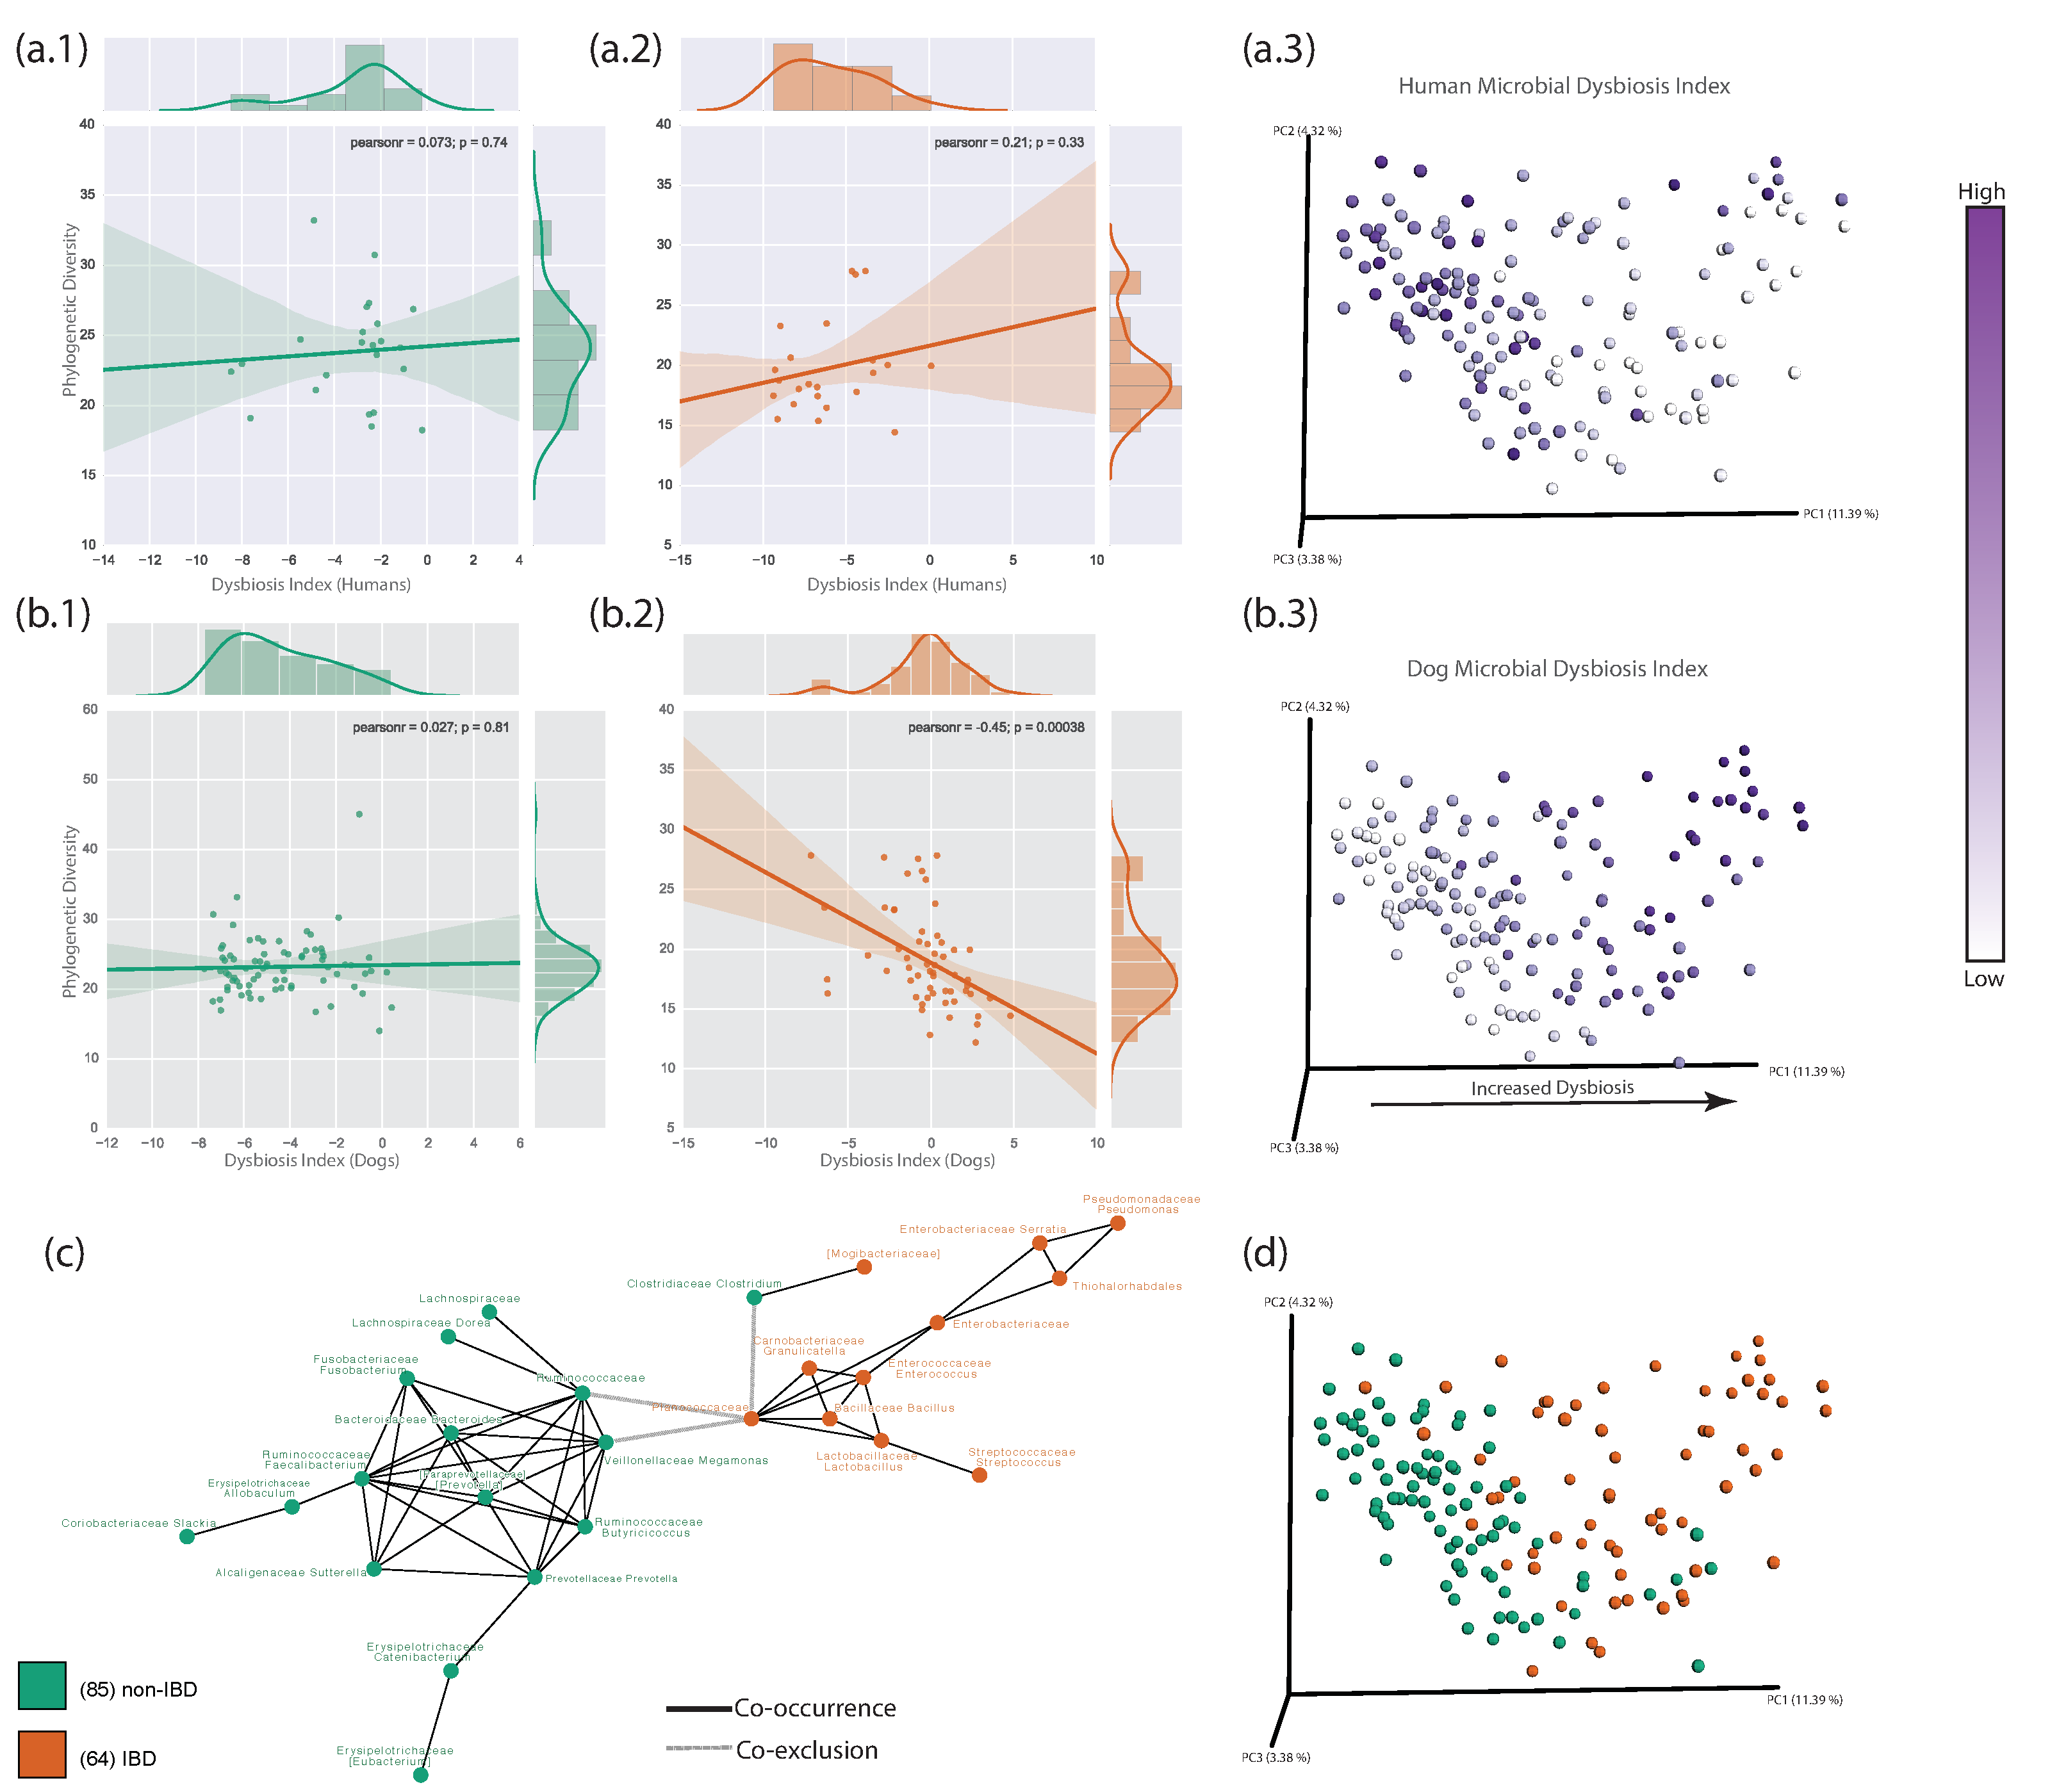
\includegraphics[width=1\columnwidth]{dogs-figures/figure-2}
\label{dogs_fig2}
\caption[Human and dog dysbiosis index.]{\textbf{Human and dog dysbiosis index.} (a.1), (a.2) Human dysbiosis index describing the dog samples grouped by disease status, (a.3) weighted UniFrac PCoA plot colored by dysbiosis index. (b.1) and (b.2) Dog dysbiosis index describing the dog samples grouped by disease state, (b.3) weighted UniFrac PCoA plot colored by dysbiosis index. (c) Correlation network used to determine the dysbiosis index in dogs, colored by the bacteria associated with IBD and non-IBD samples, co-exclusion edges are showed in dotted lines and co-occurrence edges are showed in solid lines. (d) Unweighted UniFrac PCoA plot of the dog data. Figures a.1, a.2, b.1 and b.2 all display 95\% confidence intervals.}
\end{figure}

To measure the relative effect size of host-species and \gls{ibd}, we combined humans and dogs into a single \gls{pcoa} plot, marked by clinical status (Supplementary Figure~4\footnote{\label{sup2}\url{https://images.nature.com/original/nature-assets/nmicrobiol/2016/nmicrobiol2016177/extref/nmicrobiol2016177-s1.pdf}}). We demonstrate that at a microbial level the disease effect is smaller than the host effect (human vs. dog, Supplementary Figure 4 A\textsuperscript{\ref{sup2}}). Similarly the disease effect was weaker than the species effect when analyzing PICRUSt \cite{RN17472} metagenome prediction data (\gls{permanova} test grouping samples by disease status and by host-species using a binary Jaccard matrix, p=0.001, pseudo-F by disease 14.61, pseudo-F by species 52.59, Supplementary Figure 4 B\footnote{\label{sup3}\url{https://images.nature.com/original/nature-assets/nmicrobiol/2016/nmicrobiol2016177/extref/nmicrobiol2016177-s1.pdf}}), indicating that at both the compositional and predicted functional level, species is a more significant influence on the microbial community than disease (see supplemental methods and Supplementary Figure~3\textsuperscript{\ref{sup3}}). In both dogs and humans, predicted pathways were relatively similar across \gls{ibd} and non-\gls{ibd} samples, with the most abundant pathways across both groups in both species including `housekeeping' pathways such as transporters, ABC transporters, DNA repair and recombination proteins, ribosome, purine metabolism, transcription factors, peptidases, pyrimidine metabolism, and chromosome (Supplementary Figure~5\textsuperscript{\ref{sup3}}). Although these most abundant pathways were not significantly associated with health or disease, the abundance of several lower abundance pathways was significantly different across \gls{ibd} and non-\gls{ibd} samples in dogs, see Supplementary Table~3\textsuperscript{\ref{sup3}}. No pathways were significantly higher in between disease statuses in humans.

Taken together, these results have important implications for translational medicine and for understanding \gls{ibd} in dogs. Also, the major functional gene content was conserved across non-\gls{ibd} and \gls{ibd} humans and dogs. While some significant predicted functions were identified between non-\gls{ibd} and \gls{ibd} dogs, the human sample population did not have enough non-\gls{ibd} individuals analyzed for proper statistical power. This together with previous work suggests similar functional changes within the microbiota of dogs and humans with \gls{ibd}. Previous studies have already shown that some treatment approaches to \gls{ibd} that target the microbiome are conserved across dogs and humans, such as antibiotics, dietary modulation, and probiotics. For example, specific probiotic therapy has been shown to have similar effects on fecal and mucosa-adherent microbiota and host immune response (i.e., increase of tight junction proteins, increase in beneficial mucosa-adherent bacteria) in humans, dogs, and rat models of colitis \cite{RN17583, RN17357, RN158}. 
Our study also revealed that the dysbiosis networks clearly differ in some key bacterial groups. Better understanding of the similarities in these microbial networks and functional changes may extend the abilities to test therapeutic approaches across multiple host species.

\subsection{Methods}

Naturally passed fecal samples were analyzed from 85 healthy dogs and 65 dogs with chronic signs of gastrointestinal disease and confirmed inflammatory changes on histopathology. All dogs participated in different clinical studies and leftover fecal samples were utilized for this study. The protocol for sample collection was approved by the Clinical Research Review Committee of the College of Veterinary Medicine, Texas A\&M University (CRRC\#09-06). 

Dogs with clinical signs of chronic \gls{gi} disease (i.e., vomiting, diarrhea, anorexia, weight loss, etc.) were diagnosed with idiopathic \gls{ibd} based on the\gls{wsava} criteria: (i) chronic (i.e., $>$ 3 weeks) GI signs; (ii) histopathologic evidence of mucosal inflammation; (iii) inability to document other causes of GI inflammation; (iv) inadequate response to dietary, antibiotic, and anthelmintic therapies, and (v) clinical response to anti-inflammatory or immunosuppressive agents.  Histological samples were obtained endoscopically. The clinical status of each dog was evaluated using a published clinical \gls{cibdai}. Within the \gls{ibd} dogs, 41 dogs had histological confirmed inflammation in the small intestine, 18 dogs had histological changes in both small intestine and colon, and 5 dogs had only histological changes reported in the colon. Histological changes were predominantly of lymphoplasmacytic infiltrates, with a subset of dogs also showing eosinophilic and/or neutrophilic components. The mean (SD) \gls{cibdai} for \gls{ibd} dogs was 6.4 (3.1).

Dogs were excluded if they received antibiotics within the past 2 weeks of sample collection. Data on antibiotic history was nevertheless collected: 34/65 dogs with \gls{ibd} had no history of prior antibiotics administration, while 13 dogs received antibiotics several weeks ($>$2) or months before sample collection. The remaining 18 dogs in the \gls{ibd} group had no information about prior antibiotic use. In the healthy group (n=85), 76 dogs had not received any antibiotics, and 9 dogs had a history of antibiotic use, but not within the last 2 weeks of sample collection. No technical replicates were generated in this study.

Sample and animal information (i.e., age, weight, gender, breed, duration of clinical signs, histopathology, antibiotic usage) was obtained from clinical records. Also, if the owner provided the information, the exact diet (trade name and manufacturer) fed at time of sample collection was recorded in the clinical records, and the dietary macronutrients (protein, fat, and carbohydrate content) were recorded from manufacturer's provided data on the labels.

Body weights ranged from 2.9 to 55 kg (mean 22 kg, SD: 14.9 kg), which was not significantly different from (Mann Whitney test; p=0.087) the healthy dogs (range 0.9 to 50 kg; mean 20.3 kg, SD: 10.7g). Mean age (SD) was 5.4 (3.07) in the \gls{ibd} group, which was not significantly (Mann Whitney test; p=0.311) different from healthy dogs (4.7, 3.2). There was a wide breed distribution with 37 different breeds in the \gls{ibd} group and 42 different breeds in the control group. In the \gls{ibd} group, Yorkshire terrier, German Shepherd dogs and Labrador Retrievers (n=5 each) were most commonly represented.

\Gls{bcs} were assessed according to the \gls{wsava} criteria. \Gls{bcs} is rated in a 9-point scale that visually evaluates a dog's body composition. This score has been validated against the standard \gls{dexa} \cite{RN4000}. For this dataset, the \Gls{bcs} was restricted to a subset of the healthy samples, therefore \gls{ibd} vs. Healthy comparisons could not be made in this case.

\subsubsection{DNA Extraction and Sequencing}

DNA isolation was performed as described by the Earth Microbiome Project Protocol (version 4\textunderscore 13) for 16S rRNA\cite{RN164}. The full cohort included 192 samples, of which 15 were removed because those subjects had acute hemorrhagic diarrhea, and had little clinical information available. The remaining 28 samples did not recover enough sequences after quality control including screening for low counts of reads per sample. All samples were sequenced using the Illumina HiSeq platform (2 x 100 nucleotide sequences and an index read).

\subsubsection{Data Processing}

Demultiplexed and quality controlled sequences were then clustered against the Greengenes \cite{RN165} database (release 13\textunderscore 8) using the closed reference \gls{otu} picking protocol \cite{RN81} as implemented in \gls{qiime} \cite{RN41200} 1.9.0; these processing steps were performed using the default parameters. The \gls{otu} table used for primary analysis was filtered to include only samples from subjects that presented inflammatory bowel disease or that were healthy controls. Blank samples, and subjects with diarrhea were removed. Finally the table was rarefied to normalize for sampling effort \cite{RN167} at 15,000 sequences per sample, this cutoff was selected as having the best trade-off between sequences and samples per disease status category.

Samples from \cite{RN153} were processed with the same pipeline as described above, except these were rarefied at 4,500 sequences per sample.

To address the differences in sequencing length, the combination of samples with the human dataset \cite{RN154} was preceded by trimming the sequences to an even 100 nucleotides per sequence, the rest of the pipeline was performed as described above. The same \gls{otu} picking protocol and reference database were used, therefore allowing the combination of the studies using the \gls{otu} tables. We only used the fecal samples from the human dataset.

\subsubsection{Statistical analysis}

Jupyter Notebooks \cite{RN162} with the analysis of this dataset are available on online\footnote{\url{https://www.github.com/ElDeveloper/dogs}}. Briefly, alpha and beta diversity calculations of weighted and unweighted UniFrac \cite{RN83} were performed using \gls{qiime} version 1.9.1. To assess statistical significance in these comparisons we used \gls{permanova}, grouping the samples by disease status (healthy vs \gls{ibd}), p=0.001 in both cases; pseudo-F statistics were 9.46 for unweighted UniFrac and 39.65 for weighted UniFrac. \gls{roc} curves and feature importance were calculated using Caret \cite{RN3986} and hack\textunderscore ml \footnote{\url{https://github.com/RNAer/hack_ml}}.

Statistical significance between diversity distributions were calculated using Mann-Whitney's test, linear regressions and correlation coefficients were calculated using NumPy 1.10.4 \cite{RN3823} and SciPy version 0.17, and visualized using Seaborn 0.7.0 \cite{RN170}. Principal coordinates analysis plots were created using Emperor 0.9.51-dev~\cite{RN3730}.

Metagenome predictions were performed using the Galaxy implementation of PiCRUST version 1.9.0. Significant differences in predicted KEGG Pathways between healthy and \gls{ibd} groups were calculated using a Kruskal-Wallis test with multiple corrections (FDR and Bonferroni corrected p-values). The 16S data is comprised of 85 healthy dogs, 64 \gls{ibd}-affected dogs, 29 healthy humans and 450 humans with \gls{ibd}. On the other hand the PICRUSt predicted data is comprised of 85 healthy dogs, 42 \gls{ibd}-affected dogs, 23 healthy humans and 344 humans with \gls{ibd}.

The Jaccard distance was used to compare the PICRUSt predicted data. This metric compares the samples on a presence/absence basis, and is not concerned with the similarity in the abundances of the \glspl{otu} but rather with the overlap in their presence. Each value is computed as one minus the ratio of shared \glspl{otu} to total \glspl{otu} present in the two samples.

To assess the quality of the predictions in the dog samples, we computed the `nearest sequenced taxon index' (see Supplementary Figure S3\footnote{\url{https://images.nature.com/original/nature-assets/nmicrobiol/2016/nmicrobiol2016177/extref/nmicrobiol2016177-s1.pdf}}), and verified that the samples had acceptable values (below 0.15).

\subsubsection{Dysbiosis Network}

The dysbiosis network was calculated as described in \cite{RN154}, using CCREPE \cite{RN168} and visualized using Cytoscape \cite{RN169}. The index is calculated by taking the log transform of the abundance of the ratio of \gls{ibd}-associated microbes to non-\gls{ibd} associated microbes as determined by the correlation network.

This network is created by first scoring the co-occurrence and co-exclusion patterns in the samples. CCREPE uses a compositionally adjusted version of the checkerboard score \cite{RN3985}; the results are filtered to remove non-statistically significant relationships, and to preserve the largest connected component only. We represent the results as a graph where vertices are microbes and edges are interaction types. Vertices are of one of two classes (\gls{ibd}-associated and Healthy-associated) as determined by the class where they were dominantly abundant, and edges between vertices have a weight given by their adjusted checkerboard score (negative values represent co-exclusions, and positive values represent co-occurrences). The specifics of this processing are described in the supplemental Jupyter notebooks.

\subsubsection{Accession Numbers}

Raw sequences for the dog samples have been deposited to the \gls{ena} at the following accession number ERP014919, equivalent processed \gls{otu} tables and metadata can be accessed through Qiita\footnote{\label{qiitaurl}\url{https://qiita.microbio.me}} under study 833 - `Dog models of inflammatory bowel disease'.

The data for the human dataset\cite{RN154} can be found in the \gls{ena} at the following accession numbers ERP015241 and ERP015242, equivalent processed \gls{otu} tables and metadata can be accessed through Qiita\textsuperscript{\ref{qiitaurl}} under study identifiers 1939 and 1998 -`The Treatment-Naive Microbiome in New-Onset Crohn's Disease'.

Data for the additional dog study \cite{RN153} can be found at the \gls{sra} of the under accession number SRP040310.

\subsubsection{Conflict of Interest}
We declare none.

\subsubsection{Author Contributions}
Y. V. B. wrote the manuscript, managed, interpreted and analyzed the data. E. H. contributed to the manuscript and analyzed the data. J. S. contributed to the manuscript, analyzed and interpreted the data. R. K. wrote the manuscript and interpreted the data. All authors worked together to finalize and approve this manuscript.

Please direct all material and requests to Rob Knight robknight@ucsd.edu.

\subsubsection{Acknowledgments}

We wish to acknowledge the support provided by the Crohn's and Colitis Foundation of American; the Templeton Foundation and the Keck Foundation (via the Earth Microbiome Project), the National institutes of Health. We wish to thank Zhenjiang Xu, Jon Sanders, Amnon Amir, Gail Ackermann, Jamie Morton, Luke Ursell, Jessica Metcalf, Antonio Gonzalez and Emma Schwager for their useful comments and feedback in the writing of this manuscript. 
